\documentclass[14pt]{extbook}
\usepackage{multicol, enumerate, enumitem, hyperref, color, soul, setspace, parskip, fancyhdr} %General Packages
\usepackage{amssymb, amsthm, amsmath, latexsym, units, mathtools} %Math Packages
\everymath{\displaystyle} %All math in Display Style
% Packages with additional options
\usepackage[headsep=0.5cm,headheight=12pt, left=1 in,right= 1 in,top= 1 in,bottom= 1 in]{geometry}
\usepackage[usenames,dvipsnames]{xcolor}
\usepackage{dashrule}  % Package to use the command below to create lines between items
\newcommand{\litem}[1]{\item#1\hspace*{-1cm}\rule{\textwidth}{0.4pt}}
\pagestyle{fancy}
\lhead{Progress Quiz 10}
\chead{}
\rhead{Version B}
\lfoot{1995-1928}
\cfoot{}
\rfoot{test}
\begin{document}

\begin{enumerate}
\litem{
Graph the equation below.\[ f(x) = -(x-1)^2 + 19 \]\begin{enumerate}[label=\Alph*.]
\begin{multicols}{2}\item 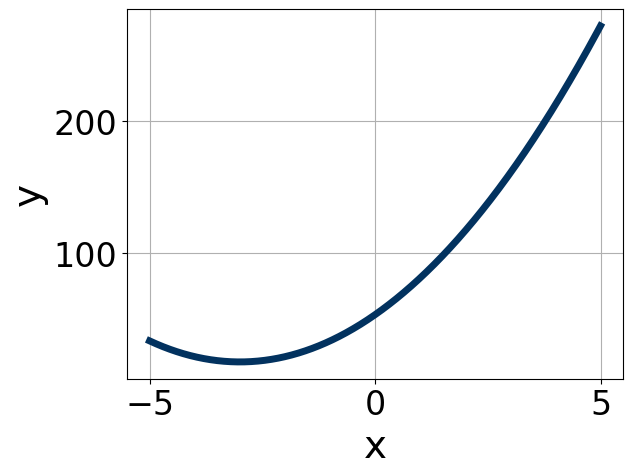
\includegraphics[width = 0.3\textwidth]{../Figures/quadraticEquationToGraphCopyAB.png}\item 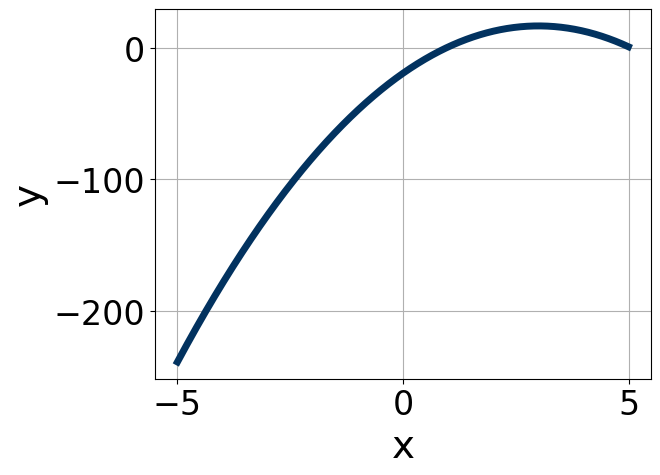
\includegraphics[width = 0.3\textwidth]{../Figures/quadraticEquationToGraphCopyBB.png}\item 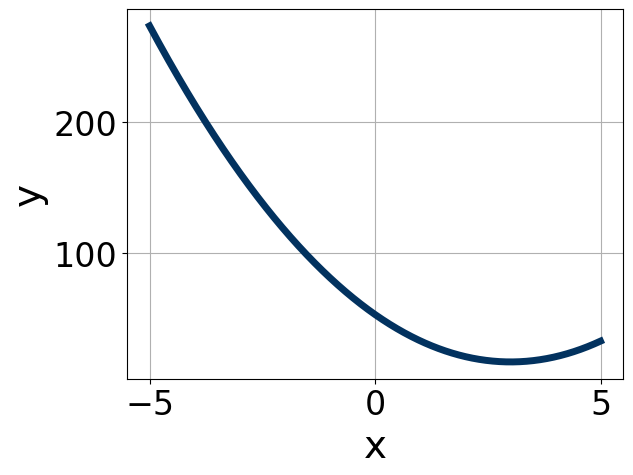
\includegraphics[width = 0.3\textwidth]{../Figures/quadraticEquationToGraphCopyCB.png}\item 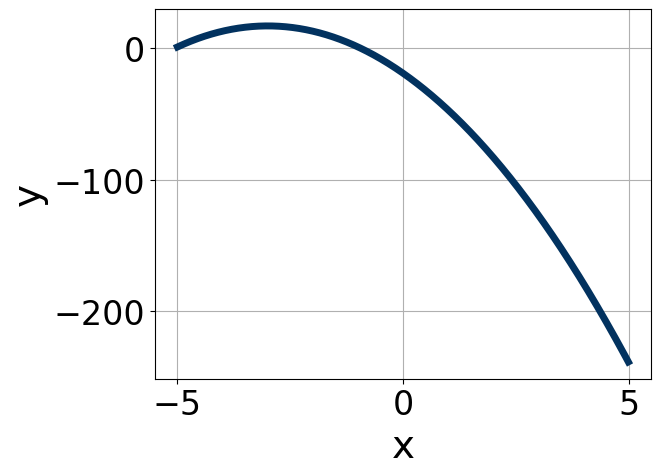
\includegraphics[width = 0.3\textwidth]{../Figures/quadraticEquationToGraphCopyDB.png}\end{multicols}\item None of the above.
\end{enumerate} }
\litem{
Solve the quadratic equation below. Then, choose the intervals that the solutions belong to, with $x_1 \leq x_2$ (if they exist).\[ 11x^{2} +8 x -2 = 0 \]\begin{enumerate}[label=\Alph*.]
\item \( x_1 \in [-2.7, -0.2] \text{ and } x_2 \in [0.03, 0.45] \)
\item \( x_1 \in [-11.9, -9.7] \text{ and } x_2 \in [1.48, 2.46] \)
\item \( x_1 \in [-12.8, -11.8] \text{ and } x_2 \in [11.45, 12.85] \)
\item \( x_1 \in [-0.8, 0.3] \text{ and } x_2 \in [0.85, 1.43] \)
\item \( \text{There are no Real solutions.} \)

\end{enumerate} }
\litem{
Factor the quadratic below. Then, choose the intervals that contain the constants in the form $(ax+b)(cx+d); b \leq d.$\[ 36x^{2} +60 x + 25 \]\begin{enumerate}[label=\Alph*.]
\item \( a \in [4.67, 7.27], \hspace*{5mm} b \in [-1, 6], \hspace*{5mm} c \in [4.3, 7.1], \text{ and } \hspace*{5mm} d \in [1, 6] \)
\item \( a \in [2.94, 3.22], \hspace*{5mm} b \in [-1, 6], \hspace*{5mm} c \in [9.3, 13.9], \text{ and } \hspace*{5mm} d \in [1, 6] \)
\item \( a \in [0.14, 1.37], \hspace*{5mm} b \in [25, 31], \hspace*{5mm} c \in [-0.7, 1.3], \text{ and } \hspace*{5mm} d \in [30, 33] \)
\item \( a \in [17.89, 18.48], \hspace*{5mm} b \in [-1, 6], \hspace*{5mm} c \in [1.7, 5.1], \text{ and } \hspace*{5mm} d \in [1, 6] \)
\item \( \text{None of the above.} \)

\end{enumerate} }
\litem{
Write the equation of the graph presented below in the form $f(x)=ax^2+bx+c$, assuming  $a=1$ or $a=-1$. Then, choose the intervals that $a, b,$ and $c$ belong to.
\begin{center}
    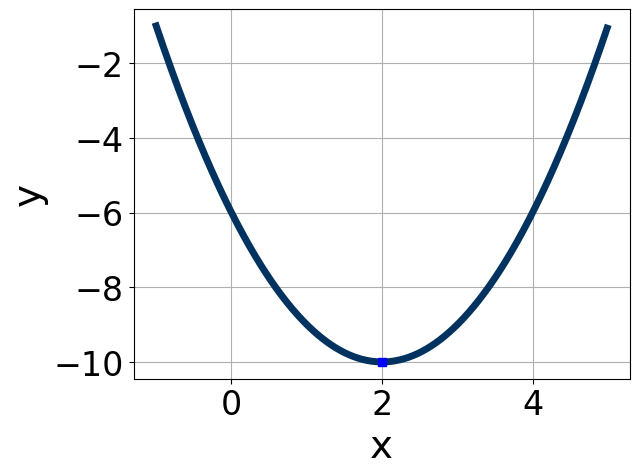
\includegraphics[width=0.5\textwidth]{../Figures/quadraticGraphToEquationCopyB.png}
\end{center}
\begin{enumerate}[label=\Alph*.]
\item \( a \in [-1.8, -0.8], \hspace*{5mm} b \in [2, 7], \text{ and } \hspace*{5mm} c \in [-5, 0] \)
\item \( a \in [-0.3, 2], \hspace*{5mm} b \in [-6, 0], \text{ and } \hspace*{5mm} c \in [-1, 3] \)
\item \( a \in [-1.8, -0.8], \hspace*{5mm} b \in [-6, 0], \text{ and } \hspace*{5mm} c \in [-5, 0] \)
\item \( a \in [-0.3, 2], \hspace*{5mm} b \in [2, 7], \text{ and } \hspace*{5mm} c \in [3, 10] \)
\item \( a \in [-0.3, 2], \hspace*{5mm} b \in [-6, 0], \text{ and } \hspace*{5mm} c \in [3, 10] \)

\end{enumerate} }
\litem{
Solve the quadratic equation below. Then, choose the intervals that the solutions $x_1$ and $x_2$ belong to, with $x_1 \leq x_2$.\[ 25x^{2} +25 x -36 = 0 \]\begin{enumerate}[label=\Alph*.]
\item \( x_1 \in [-47.4, -42.3] \text{ and } x_2 \in [19.99, 20.18] \)
\item \( x_1 \in [-2.9, -1.2] \text{ and } x_2 \in [0.78, 0.89] \)
\item \( x_1 \in [-11.9, -8.9] \text{ and } x_2 \in [0.1, 0.18] \)
\item \( x_1 \in [-7.8, -3.8] \text{ and } x_2 \in [0.18, 0.35] \)
\item \( x_1 \in [-1.1, 0.4] \text{ and } x_2 \in [1.54, 1.78] \)

\end{enumerate} }
\litem{
Factor the quadratic below. Then, choose the intervals that contain the constants in the form $(ax+b)(cx+d); b \leq d.$\[ 54x^{2} -57 x + 10 \]\begin{enumerate}[label=\Alph*.]
\item \( a \in [-0.41, 1.86], \hspace*{5mm} b \in [-49, -41], \hspace*{5mm} c \in [0, 2.5], \text{ and } \hspace*{5mm} d \in [-15, -9] \)
\item \( a \in [1.79, 2.44], \hspace*{5mm} b \in [-9, -1], \hspace*{5mm} c \in [25.8, 27.1], \text{ and } \hspace*{5mm} d \in [-2, 2] \)
\item \( a \in [17.05, 18.7], \hspace*{5mm} b \in [-9, -1], \hspace*{5mm} c \in [1.5, 3.1], \text{ and } \hspace*{5mm} d \in [-2, 2] \)
\item \( a \in [4.82, 6.09], \hspace*{5mm} b \in [-9, -1], \hspace*{5mm} c \in [7.7, 11], \text{ and } \hspace*{5mm} d \in [-2, 2] \)
\item \( \text{None of the above.} \)

\end{enumerate} }
\litem{
Solve the quadratic equation below. Then, choose the intervals that the solutions belong to, with $x_1 \leq x_2$ (if they exist).\[ 15x^{2} +7 x -6 = 0 \]\begin{enumerate}[label=\Alph*.]
\item \( x_1 \in [-0.85, 0.51] \text{ and } x_2 \in [0.6, 1.1] \)
\item \( x_1 \in [-21.23, -19.29] \text{ and } x_2 \in [19, 20.2] \)
\item \( x_1 \in [-0.96, -0.79] \text{ and } x_2 \in [-0.5, 0.6] \)
\item \( x_1 \in [-14.25, -13.19] \text{ and } x_2 \in [5.2, 7.2] \)
\item \( \text{There are no Real solutions.} \)

\end{enumerate} }
\litem{
Solve the quadratic equation below. Then, choose the intervals that the solutions $x_1$ and $x_2$ belong to, with $x_1 \leq x_2$.\[ 8x^{2} +18 x -81 = 0 \]\begin{enumerate}[label=\Alph*.]
\item \( x_1 \in [-7.5, -3.5] \text{ and } x_2 \in [1.77, 2.46] \)
\item \( x_1 \in [-1.5, 3.5] \text{ and } x_2 \in [6.02, 7.51] \)
\item \( x_1 \in [-9, -7] \text{ and } x_2 \in [0.81, 1.17] \)
\item \( x_1 \in [-14.5, -9.5] \text{ and } x_2 \in [-0, 0.87] \)
\item \( x_1 \in [-40, -30] \text{ and } x_2 \in [17.2, 18.23] \)

\end{enumerate} }
\litem{
Write the equation of the graph presented below in the form $f(x)=ax^2+bx+c$, assuming  $a=1$ or $a=-1$. Then, choose the intervals that $a, b,$ and $c$ belong to.
\begin{center}
    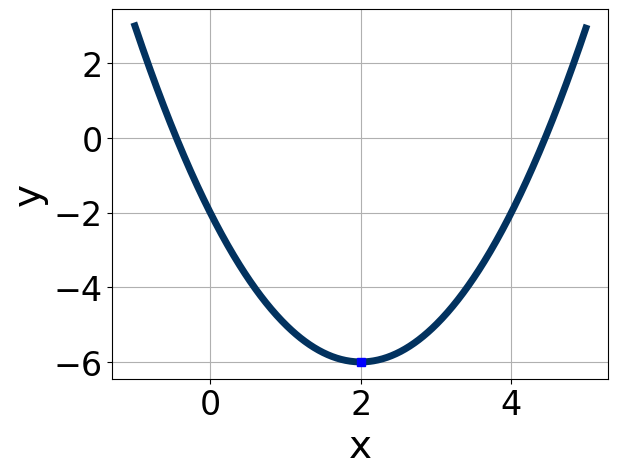
\includegraphics[width=0.5\textwidth]{../Figures/quadraticGraphToEquationB.png}
\end{center}
\begin{enumerate}[label=\Alph*.]
\item \( a \in [1, 7], \hspace*{5mm} b \in [-5, -1], \text{ and } \hspace*{5mm} c \in [-7, -3] \)
\item \( a \in [-2, 0], \hspace*{5mm} b \in [2, 8], \text{ and } \hspace*{5mm} c \in [-12, -10] \)
\item \( a \in [-2, 0], \hspace*{5mm} b \in [-5, -1], \text{ and } \hspace*{5mm} c \in [4, 7] \)
\item \( a \in [-2, 0], \hspace*{5mm} b \in [-5, -1], \text{ and } \hspace*{5mm} c \in [-12, -10] \)
\item \( a \in [1, 7], \hspace*{5mm} b \in [2, 8], \text{ and } \hspace*{5mm} c \in [-7, -3] \)

\end{enumerate} }
\litem{
Graph the equation below.\[ f(x) = (x-4)^2 - 16 \]\begin{enumerate}[label=\Alph*.]
\begin{multicols}{2}\item 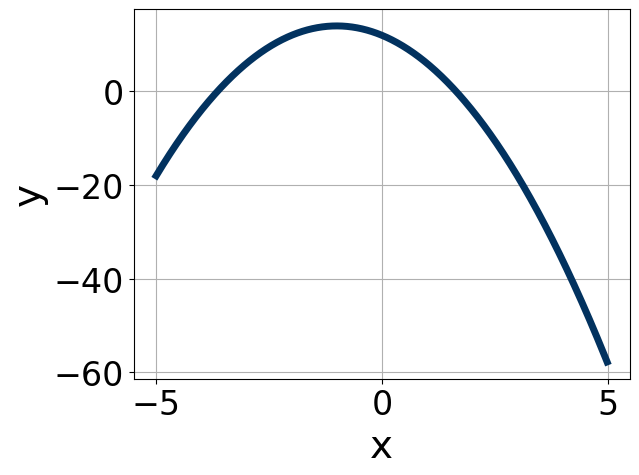
\includegraphics[width = 0.3\textwidth]{../Figures/quadraticEquationToGraphAB.png}\item 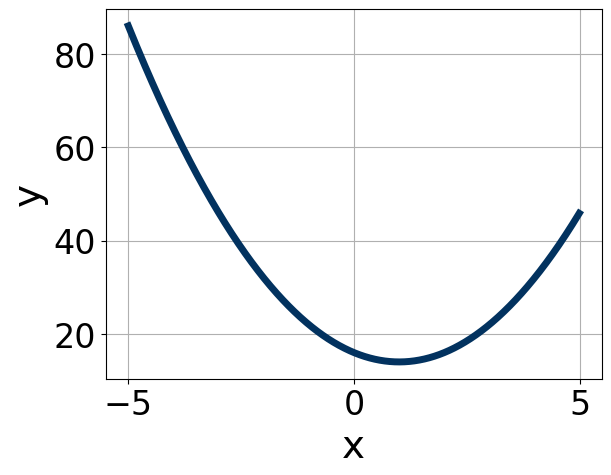
\includegraphics[width = 0.3\textwidth]{../Figures/quadraticEquationToGraphBB.png}\item 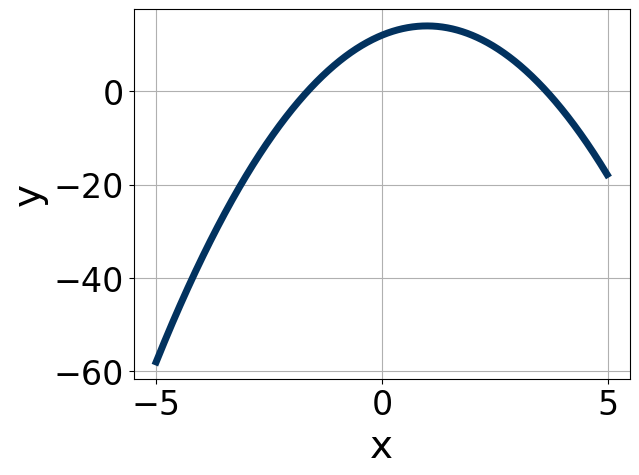
\includegraphics[width = 0.3\textwidth]{../Figures/quadraticEquationToGraphCB.png}\item 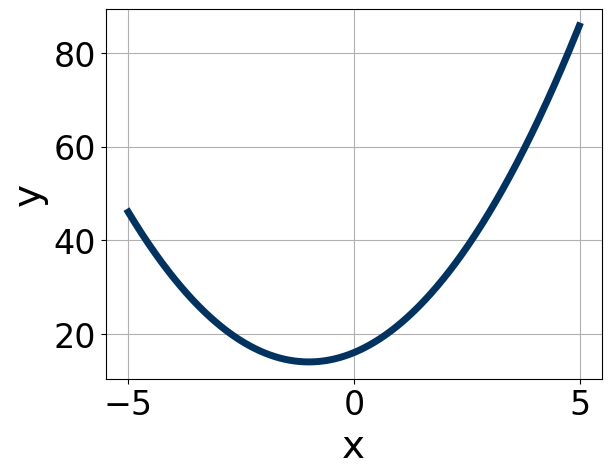
\includegraphics[width = 0.3\textwidth]{../Figures/quadraticEquationToGraphDB.png}\end{multicols}\item None of the above.
\end{enumerate} }
\end{enumerate}

\end{document}